\subsection{Describe how the Stern-Gerlach experiment led to the discovery of the spin of the electron. Which properties does the spin possess?}


Stern-Gerlach eksperimentet blev udført af Stern og Gerlach i 1921, og skulle bekræfte Bohr-Sommerfeld teorien om, at impulsmoment er kvantiseret.

\paragraph{Opstillingen:} Eksperimentet, som kan ses på \cref{fig:Q08_SternGerlachEksperimentOpstilling}, benytter en kollimeret stråle af sølvatomer, siden disse er tunge og neutralt ladede partikler, så man skulle ikke bekymre sig om en Lorentzkraft, som kunne afbøje partiklerne, i stedet for at vise, at partiklerne blev afbøjet relativit til deres formodede kvantiseret impulsmoment, hvor sidstnævnte ønskedes værende den dominerende faktor for resultatet af eksperimentet. Disse atomer blev sendt gennem et inhomogent magnetfelt skabt af en magnet, hvilket afbøjer atomerne grundet deres magnetiske dipolmoment, som skabes af deres impulsmoment, og dette danner et mønster på den fotografiske plade for enden af strålen (udenfor magneten).

\begin{figure}[!h]
    \centering
    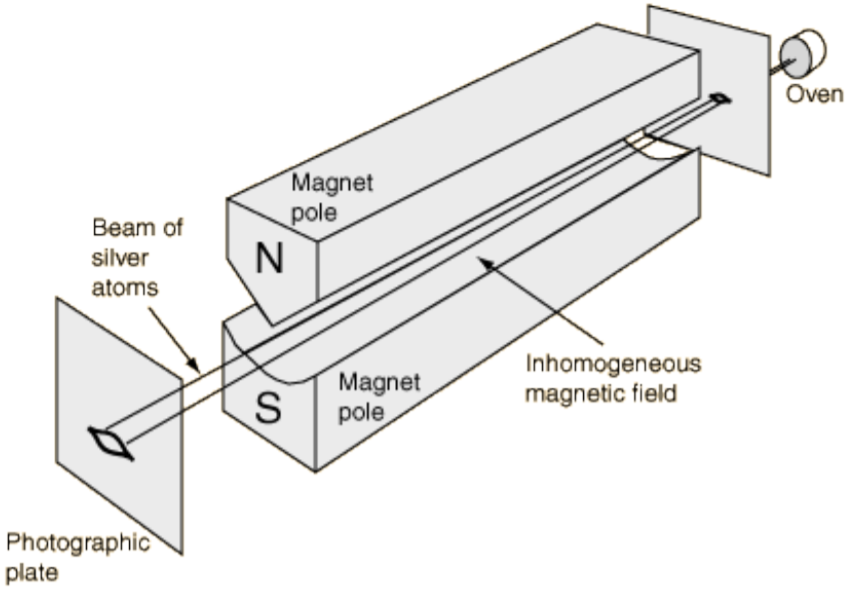
\includegraphics[width = .75\textwidth]{Q08/images/SternGerlachExperiment.PNG}
    \caption{Opstillingen af Stern-Gerlach eksperimentet.}
    \label{fig:Q08_SternGerlachEksperimentOpstilling}
\end{figure}

\paragraph{Forventning vs. resultat:} Eksperimentet havde mulighed for flere udfald, alt efter hvilken teori, som man anså som rigtig, se \cref{fig:Q08_SternGarlachExperimentResult}. Både den klassiske og den kvantemekaniske fortolkning var enige om, at var det totale impulsmoment $l = 0$, så ville det ikke interagere med det magnetiske felt, hvorfor atomerne blot ville fortsætte uden at blive afbøjet, og det samme ville gøre sig gældende, hvis der intet magnetfelt var. For impulsmomenter forskellig fra nul -- hvilket man i 1921, hvor eksperimentet blev udført, var sikker på, da man mente, at det havde $L = 1$ -- var de to teorier dog ikke enige.

Lamors klassiske teori om, at der ikke var en foretrukken retning for en magnetisk dipol, som man kan se et atom som, formodede, at man ville se et ''udsmurt'' mønster mellem den maksimale positive og negative afbøjning -- der ville fremkomme, når atomets magnetisk dipol ville være hhv. parallel og anti-parallel med $z$-aksen -- på den fotografiske plade, dog med maksimal intensitet i midten af sølvatomstrålen.

I Bohr-Sommerfeld teorien var impulsmomenter kvantiseret, hvorfor man for et totalimpulsoment for sølv på $L = 1$ ville se sølvatomerne blive afbøjet i 3 forskellige retnigner: Én for maksimal positiv afbøjning, én for maksimal negativ afbøjning, og én for ingen afbøjning.

Eksperimentets udfald viste sig dog at være noget anderledes. Der var en vis lighed mellem resultatet og Bohr-Sommerfeld teorien, idet atomerne fordelte sig, som havde det kvantiserede impulsmomenter, men der blev dog kun observeret \emph{to} og ikke \emph{tre} afbøjninger, som forventet, se \cref{fig:Q08_SternGarlachExperimentResult}.

\begin{figure}[!h]
    \centering
    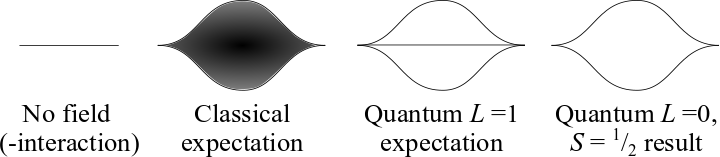
\includegraphics[width=\textwidth]{Q08/images/SternGerlachExperimentResult.png}
    \caption{Fra venstre mod højre: Hvis der ikke var et magnetisk felt, eller hvis der ikke var interaktion med dette felt (totalt impulsmoment lig $0$); den klassiske formodning baseret på Larmors klassiske teori om, at en magnetiske dipol ikke har en foretrukken retning; den kvantemekaniske formodning baseret på Bohr-Sommerfelt teorien om, at impulsmoment er kvantiseret, og den daværende viden om, at sølv havde $L = 1$; det faktiske resultat fra Stern-Garlach eksperimentet, som viser $J = 1/2$, da sølv faktisk har $L = 0$, men har spin $S = 1/2$.}
    \label{fig:Q08_SternGarlachExperimentResult}
\end{figure}

Det blev foreslået af Uhlenbeck og Goudsmit i 1925, at elektroner havde et indre impulsmoment, også kaldet spin, hvilket viste sig at være rigtigt og kunne forklare resultatet fra Stern-Gerlach eksperimentet.
\noindent
Det viste sig, at \ldots


\paragraph{Egenskaber ved spin:} Spin er et impulsmoment, hvorfor det vil kunne beskrives ved de samme vektoregenskaber som vi kender fra baneimpulsmomentet $L$, hvor egenvektorerne for $\Vec{S}^2$ og $\Vec{S}_z$ vil være givet ved
\begin{align}
    \Vec{S}^2\ket{S \: m_S} &= \hbar^2 S(S+1) \ket{S \: m_S} \label{eq:Q08_EgenvektorligningForS^2} \: , \\
    \Vec{S}_z\ket{S \: m_S} &= \hbar m_S \ket{S \: m_S} \: , \label{eq:Q08_EgenvektorligningForS_z}
\end{align}
hvorfra man kan finde egenskaben for ''spin-stepopreratorerne''
\begin{align}
    \Vec{S}_\pm \ket{S \: m_S} &= \hbar \sqrt{S(S+1) - m_S(m_S \pm 1)} \ket{S \: (m \pm 1)} \: , \quad \Vec{S}_\pm \equiv \Vec{S}_x \pm i \Vec{S}_y \: .
\end{align}
\noindent
Modsat baneimpulsmomentet må spin dog gerne have halve værdier for $S$ (i værdier af $\hbar$) og $m_S$, så
\begin{align}
    S &= 0, \: \frac{1}{2}, \: 1, \: \frac{3}{2}, \: \ldots \: , \\
    m_S &= -S, \: -S + 1, \: \ldots \: , \: S - 1, \: S \: .
\end{align}

Alle elementarpartikler har et specifik spin: $\pi$-mesoner har spin $0$; elektroner, neutroner og protoner har spin $1/2$; fotoner har spin $1$; $\Delta$-baryoner har spin $3/2$; gravitroner har spin $2$; osv..

\noindent
For en elektron vil man derfor få absolutværdien af spinvektoren, fra \cref{eq:Q08_EgenvektorligningForS^2},
\begin{align}
    \| \Vec{s} \| &= \sqrt{\hbar^2 \frac{1}{2}\left(\frac{1}{2}+1\right)} = \sqrt{\frac{3}{4}}\hbar  \: , \\
\end{align}
og de to komponenter i $z$-retninger er, fra \cref{eq:Q08_EgenvektorligningForS_z},
\begin{align}
    s_z &= \hbar \left(\pm \frac{1}{2}\right) = \pm \frac{1}{2}\hbar \: ,
\end{align}
hvilket kan ses på \cref{fig:Q08_PropertiesOfSpin}.

\begin{figure}[!h]
    \centering
    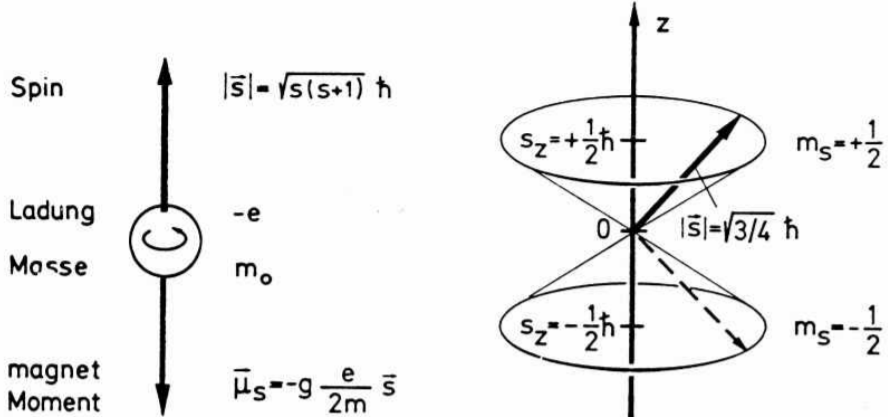
\includegraphics[width=\textwidth]{Q08/images/ProportiesOfSpin.PNG}
    \caption{Egenskaber ved spin for en elektron.}
    \label{fig:Q08_PropertiesOfSpin}
\end{figure}
$ $\\

For alle fermioner gør Paulis eksklusionsprincip sig gældende. Dette siger, at to fermioner kan ikke have de samme kvantetal, hvilket for elektroner betyder, at der maksimalt kan være to elektroner i hver orbital, da disse vil have hhv. spin-op og spin-ned, og dermed ikke have det samme $m_s$ kvantetal. Dette viser også, at hvis vi har 2 elektroner i en samme orbital, så vil deres spin gå ud med hinanden og resulterer, hvilket i Stern-Garlach eksperimentet ville resultere i et mønster som formodningen, når der ikke var en felt-interaktion, \cref{fig:Q08_SternGarlachExperimentResult}(længst til venstre), da denne er afhængig af $m_S$, \cref{ }.